\def\width{16}
\def\hauteur{16}
%
%
%

\definecolor{orange}{RGB}{250,230,200}
\definecolor{gray}{RGB}{220,220,220}
\definecolor{pink}{RGB}{247,206,205}

\begin{figure}[t]
\vspace{-2mm}
    \centering
        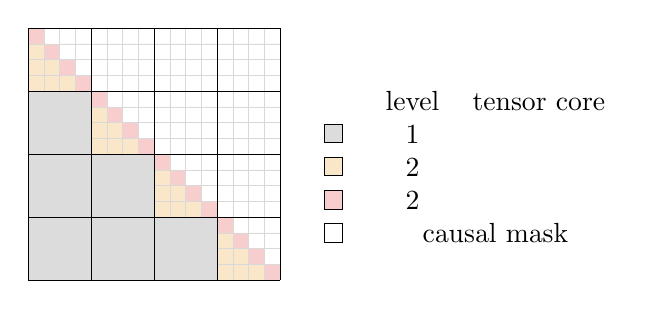
\begin{tikzpicture}[x=0.2cm, y=0.2cm]
    %
    %
    
    %
    %
    %

    \foreach \y in {0, ..., 15}{
        \foreach \x in {0, ...,  15} {%
        %
            \pgfmathsetmacro{\col}{ifthenelse(\x<15-\y,"orange",ifthenelse(\x==\y+1,"white","white"))}
       \fill[\col] (\x,\y) rectangle (\x+1,\y+1);
       }
    }
    \foreach \y in {0, ..., 15}{
       \fill[pink] (\y,15-\y) rectangle (\y+1,15-\y+1);
       }
    
   
    \draw[step=0.20cm, line width=0.05mm, black!15!white, fill=orange] (0,0) grid (\width,\hauteur);
    \foreach \x in {0, ..., 8} {%
    %
    \fill[gray] (\x,0) rectangle (\x+4,4);
    }
        \foreach \x in {0, ..., 4} {%
    %
    \fill[gray] (\x,4) rectangle (\x+4,8);
    }
    \foreach \x in {0, ..., 1} {%
    %
    \fill[gray] (\x,8) rectangle (\x+3,12);
    }
    
    \foreach \x in {0, ..., 1} {%
    %
    \fill[gray] (\x,8) rectangle (\x+3,12);
    }


    \draw[step=0.8cm, line width=0.1mm, black!10!black, fill=orange] (0,0) grid (\width,\hauteur);

    %
    %
    %
      
    %
    %
    %
    %
        \node 
        [shape=rectangle,fill=white, 
        align=center](table2) at (28.0,7.0) {

            \begin{tabular}{lcc} \toprule
                 & level & tensor core   \\ 
            \begin{tikz}
                \node [draw,fill=gray] {};
            \end{tikz} & 1 & $\checkmark$\\
                \begin{tikz}
                \node [draw,fill=orange] {}; 
            \end{tikz} & 2 & $\checkmark$\\
             \begin{tikz}
                \node [draw,fill=pink] {}; 
            \end{tikz} & 2 & $\text{\xmark}$\\
                 \begin{tikz}
                \node [draw,fill=white] {}; 
            \end{tikz} & \multicolumn{2}{ c}{causal mask}\\
                 %
                \bottomrule
            \end{tabular}
        };

%
    \end{tikzpicture}
\vspace{-2mm}
    \caption{
    Attention-style map to illustrate the chunkwise computations in GLA. The inter-chunk dependencies (in gray) 
    are not directly computed in the chunkwise form (only computed in the parallel form).
    The intra-chunk dependencies are modeled via secondary chunking/tiling where the inter-sub-chunk part (in orange) is computed by half-precision matmuls while the intra-sub-chunk part (in pink) is computed in full precision in log space. 
    }
    \label{fig:gla_tiling}

\end{figure}
